Ein kinounternehmen besitzt mehrere Kinos mit Namen.
Jedes Kino hat mehrere durchnummerierte Säle.\\
Erstellen Sie das Domänenmodell inclusive Attributen und Multiplizitäten.


\section*{Antwort}

S. Abbildung~\ref{fig:kino}.\\


\noindent
Die Multiplizität der \code{Unternehmen} - \code{Kino} Assoziation wurde mit \code{*}\footnote{
    ``A multiplicity with zero as the lower bound and an unspecified upper bound may use the alternative notation containing a single star `*` instead of `0..*`
    multiplicity.`` (\cite[35]{UML17})
} angegeben.\\
Zwar geht aus den Anforderungen hervor, dass ein Unternehmen \textit{mehrere} Kinos betreibt.
Aber eine alternative Multiplizität von \code{1..*} würde bedeuten, dass ein Unternehmen immer mindestens ein Kino betreiben muss und demnach auch nur existieren kann, wenn ein assoziiertes \code{Kino} existiert\footnote{
vgl. ``\textit{Muss-Beziehung}``, \cite[166 ff.]{Bal05}
}.\\
Wir gehen davon aus, dass in dem späteren Softwaresystem ein der Fachlichkeit entsprechendes Unternehmen auch ohne \code{Kino} existieren kann.


\begin{figure}
    \centering
    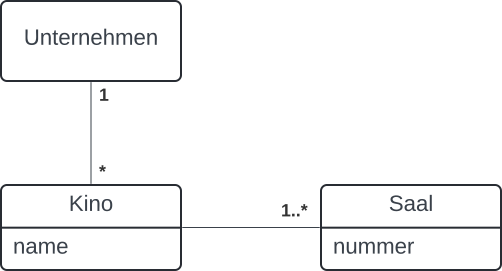
\includegraphics[scale=0.4]{chapters/aufgabe 2/img/kino}
    \caption{Domänenmodell für Aufgabe 2. (Quelle: eigene)}
    \label{fig:kino}
\end{figure}